\documentclass[../summary.tex]{subfiles}

\begin{document}
	
	\section{Economics for sustainability}
	
	\subsection{Study guide}
	
	The study guide for chapter 10 of the MOOC was a complete mess. That is why, even though this part of the summary is still based on the study guide, there won't be an overview of it in this summary.
	\\\\
	Typical questions are:
	\begin{itemize}
		\item Definitions, terminology: be able to explain the definition, give examples
		\item Graphs: be able to explain and interpret the graphs
		\item Principles: be able to explain, give examples
	\end{itemize}
	
	\subsection{Gross Domestic Product}
	
	The Gross Domestic Product or GDP is a measure of total production that is used to reflect the economic health of a country or region and has strongly increased since the end of the 19th century. Figure \ref{fig:GDP} shows this exponential growth.
		
	\begin{figure}[htbp]
		\centering
		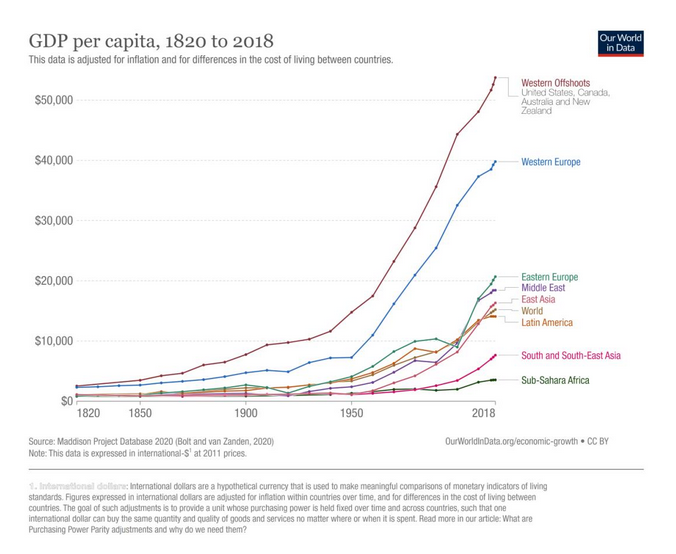
\includegraphics[width=1\linewidth]{images/10-GDP-increase.png}
		\caption{Increase in GDP since 19th century}
		\label{fig:GDP}
	\end{figure}
	
	\newpage
	This increase in GDP went together with a lot of other positive phenomena, such as an increase in life expectancy, an increase in literacy, a decrease in hunger, and so on. However, at the same time, we also saw a rise in environmental pressures, such as greenhouse gas emissions, global warming, plastic pollution, declining biodiversity, and many more. 
	\\\\
	Economic growth is the annual percentage change of real GDP. Real GDP means it's GDP measured in monetary terms but it's corrected for inflation and price changes.
	\\\\
	There are multiple ways to define GDP. The first approach is the so-called added value approach. We define GDP as the value of all final goods and services that are produced in a given country in a given period of time. A second way to define GDP is to look at incomes. All that value added in the GDP is giving rise to incomes, incomes to the persons who own the factors of production. Factors of production are labour, capital and land. So in the second approach to GDP, the income approach, GDP can be defined as the sum of all the incomes that are earned by the owners of factors of production in a given year, in a given country. 
	\\\\
	We should look at GDP as a measure of production and of economic activity. It was not intended to be a measure of prosperity or well-being or happiness. So a lot of things are not picked up by the concept of GDP. A first example of something that is missing in the GDP is a good idea about the distribution or the inequality. A second thing which is missing from the GDP is unpaid work. A third element that is not included in the GDP are changes in the quality of the environment.
	\\\\	
	Figure \ref{fig:emissions-and-GDP-per-capita} shows the emissions and GDP per capita for the different countries. Looking at the graph, we can see there seems to be an increasing relationship between GDP per capita and emissions per capita. Richer countries, with a higher GDP per capita, have higher emissions per capita. We can also see that the big countries, like China and India, are on an intermediate level of emissions. If we study the evolution of the emissions versus the GDP per capita during the 20th and 21st century, we notice two different trends. Countries like China and India started at a low level of both emissions and GDP per capita, but they gradually increased over time and are still increasing. On the other hand, we have countries like Belgium and the United States that started increasing at an intermediate level of emissions per capita, but then reached a peak and started decreasing. This pattern is observed for many developed economies and the idea behind it is the so-called Kuznets curve
	
	\begin{figure}[htbp]
		\centering
		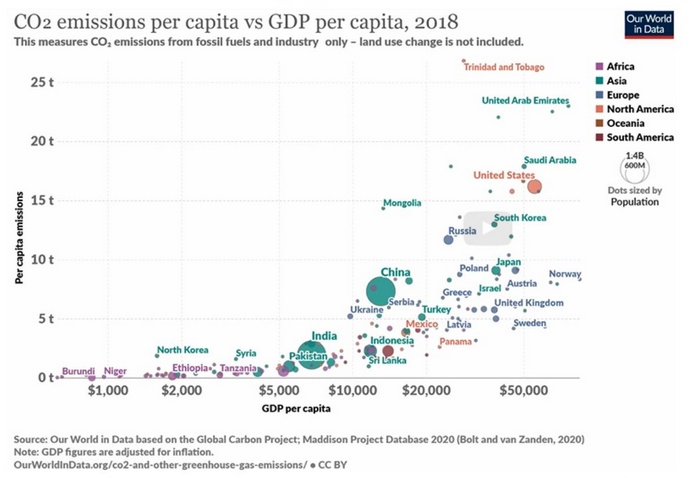
\includegraphics[width=0.9\linewidth]{images/10-emissions-and-GDP-per-capita.png}
		\caption{$CO_{2}$ emissions per capita versus GDP per capita, 2018}
		\label{fig:emissions-and-GDP-per-capita}
		
	\end{figure}
	
	\begin{figure}[htbp]
		\centering
		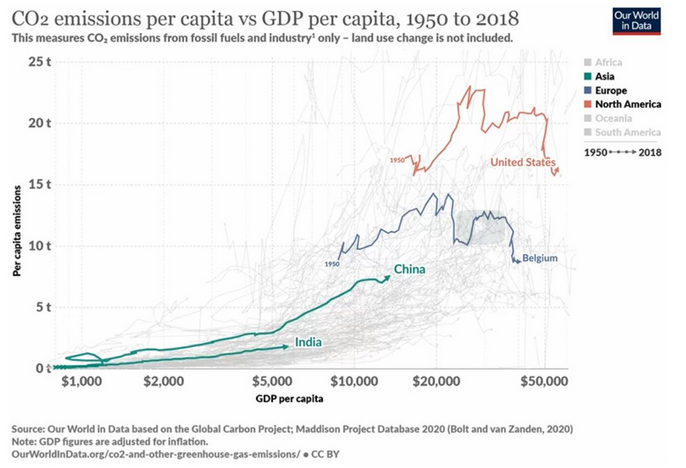
\includegraphics[width=0.9\linewidth]{images/10-emissions-and-GDP-per-capita-long-term.png}
		\caption{$CO_{2}$ emissions per capita versus GDP per capita, 1950 to 2018}
		\label{fig:emissions-and-GDP-per-capita-long-term}
		
	\end{figure}
	
	\subsection{The Kuznets curve}
	
	
	
\end{document}